\section{Mengenal .tex}
Pertama pahami dulu bagaimana badan isi file .tex yang akan kita kerjakan. Download atau lihat salah satu file latex yang akan kita kerjakan. Untuk mengisi latex kita harus mengisinya di dalam komponen  yang merupakan tag dengan pembuka begin dan diakhiri dengan end.
Kemudian kenali bagian buku terdiri dari part, chapter dan section. Part itu bisa kita andaikan bab, chapter sub bab, dan section adalah bagian.

Kita bisa memisahkan isi dari latex dengan perintah input kemudian di dalam kurung kurawal letak file .tex yang akan kita masukkan kedalam file utama latex tersebut.

LATEX merupakan program pengolahan kata atau sistem persiapan pembuatan dokumen untuk pengetikan sistem TeX, yang dinamakan berdasarkan gaya penulisannya sebagai LaTeX. Nama LaTeX itu sendiri hanya mengacu pada bahasa penulisan yang digunakan pada sebuah dokumen, bukan pada editor yang digunakan untuk menulis dokumen tersebut. Untuk membuat dokumen dalam format LaTeX, sebuah file berformat .tex harus dibuat menggunakan semacam text editor. Walaupun, banyak text editor yang dapat digunakan untuk membuat dokumen LaTeX, beberapa text editor sengaja dibuat khusus untuk menggunakan bahasa LaTex.
\subsection{Keuntungan Latex}
\begin{enumerate}
  \item Tersedianya beberapa program untuk melihat hasil pemrosesan latex yang dapat menampilkannya persis seperti hasil cetakan dengan printer
  \item Penulisan rumus matematis dapat dilakukan dengan cara sangat mudah dan profesional
  \item Banyak jurnal internasional yang menerima artikel artikel dalam format tex
  \item Pemakai hanya perlu belajar sedikit perintah yang mudah dipahami yang menyatakan struktur logis sebuah dokumen
  \item Latex mendorong pengarang untuk menulis naskah yang tersusun dengan baik
\end{enumerate}

\section{Compiler}
Kemudian untuk dapat menuliskan kode LaTex kita harus menggunakan editor LaTex. Oleh karena itu pastikan kita sudah meng-install aplikasi editor LaTex seperti texworks, texmaker, winedt dll. Untuk dapat melihat perintah yang sudah kita lakukan, kita harus melakukan compile. Compile merupakan proses eksekusi yang dilakukan untuk melihat hasil dari perintah yang telah kita buat dalam LaTex yang dapat kita preview dalam bentuk file dengan ekstensi PDF. Editor LaTex yang saya praktekkan disini adalah texmaker.


TexMaker merupakan salah satu perangkat lunak IDE, yang berlisensi GNU/GPL yang dibuat untuk mempermudah proses sebuah dokumen seperti tesis, penelitian dll. Kita bisa melakukan kompilasi dengan perintah yang ada di listing \ref{lst:compile}.

\begin{lstlisting}[caption=Perintah kompilasi latex keluaran pdf,label={lst:compile},language=sh]
pdflatex -shell-escape -interaction=nonstopmode -file-line-error git.tex | grep ".*:[0-9]*:.*|LaTeX Warning:"

pdflatex -shell-escape -interaction=nonstopmode -file-line-error git.tex | grep ".*:[0-9]*:.*"

pdflatex -shell-escape -interaction=nonstopmode -file-line-error git.tex | grep -i ".*:[0-9]*:.*\|warning"
\end{lstlisting} 

\section{Hello LATEX}
Sekarang Kamu sudah mempunyai distribusi LATEX yang sudah terinstal. Mari kita coba jalankan! Pertama buka editor Latex dan simpan file dengan nama hello.tex seperti pada listing \ref{lst:hello}.
\lstinputlisting[caption=Contoh listing kode hello Latex,label={lst:hello}]{src/0/hello.tex}\cite{kline2018latex}

\section{Mengedit Menggunakan Editor LaTex}
Editor khusus pada LaTex dibutuhkan agar kita dapat mengedit sebuah dokumen. Dengan menggunakan Editor Latex kita dapat mengedit sebuah file dokumen lalu kita dapat melihat langsung hasil dari perintah yang telah dilakukan dalam bentuk PDF. Bagaimana cara mengedit sebuah file pada LaTex? Berikut penjelasannya : 
\begin{enumerate}
\item Pertama pastikan anda telah meng-install Editor latex yang akan digunakan (Editor latex yang digunakan disini adalah TeXworks)
\item Buka Editor latex yang sudah kalian install \ref{fig:openeditor}
  \begin{figure}[!htbp]
  \centering
  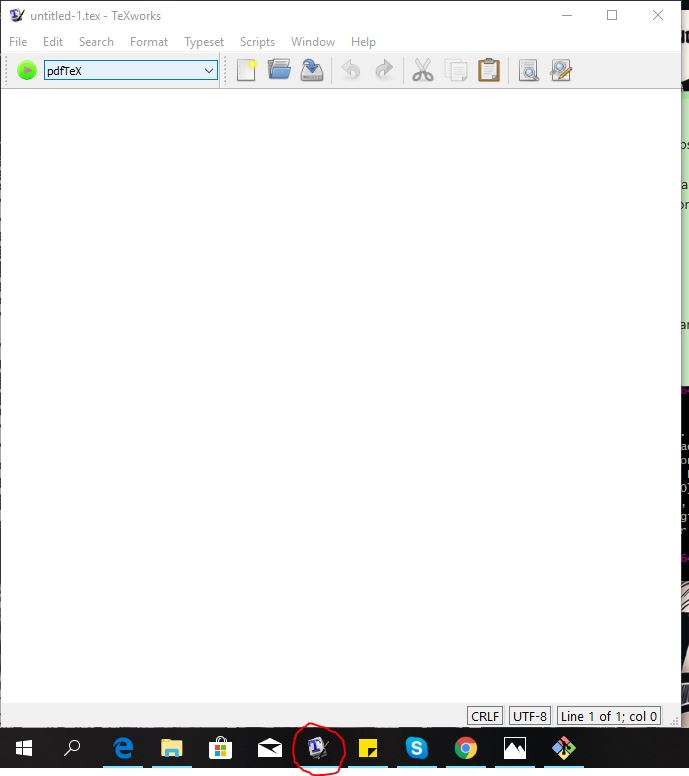
\includegraphics[width=.75\textwidth]{figures/openeditor.JPG}
  \caption{Buka Editor Latex}\label{fig:openeditor}
\end{figure}
\item Setelah membuka editor latex, pastikan terlebih dulu anda telah memiliki file atau dokumen yang akan anda edit. 
\item Kemudian, pilih menu file dan buka menu open file seperti pada gambar \ref{fig:openfile}
  \begin{figure}[!htbp]
  \centering
  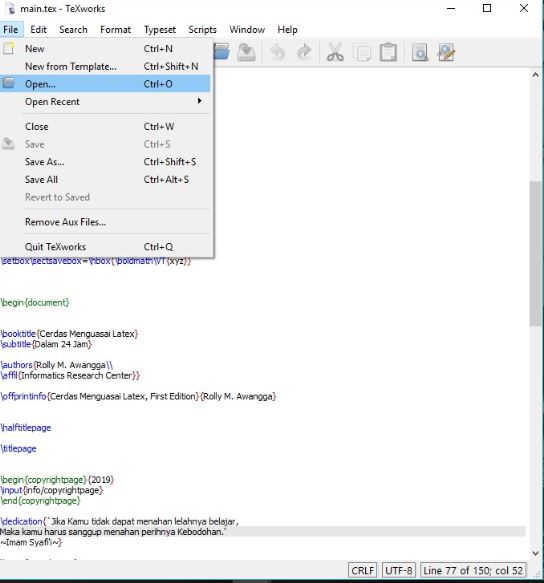
\includegraphics[width=.75\textwidth]{figures/openfile.JPG}
  \caption{Open File}\label{fig:openfile}
\end{figure}
\item Setelah memilih menu file kemudian buka file main.tex seperti pada gambar \ref{fig:openfolder}, kemudian pilih file \textbf{main.tex}
\begin{figure}[!htbp]
  \centering
  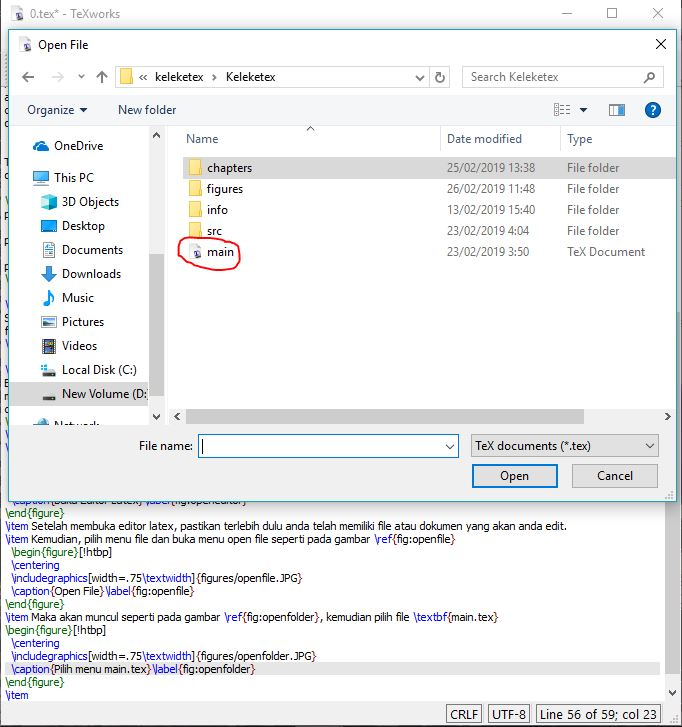
\includegraphics[width=.75\textwidth]{figures/openfolder.JPG}
  \caption{Pilih file main.tex}\label{fig:openfolder}
\end{figure}
\item Main.tex merupakan file utama dalam sebuah dokumen atau laporan ilmiah yang berisi file-file tambahan dari direktori lain. Jika anda membuka file main.tex, maka kita dapat melihat hasil atau isi dari laporan dalam bentuk preview beresktensi PDF pada main.pdf seperti pada gambar \ref{fig:main}
  \begin{figure}[!htbp]
  \centering
  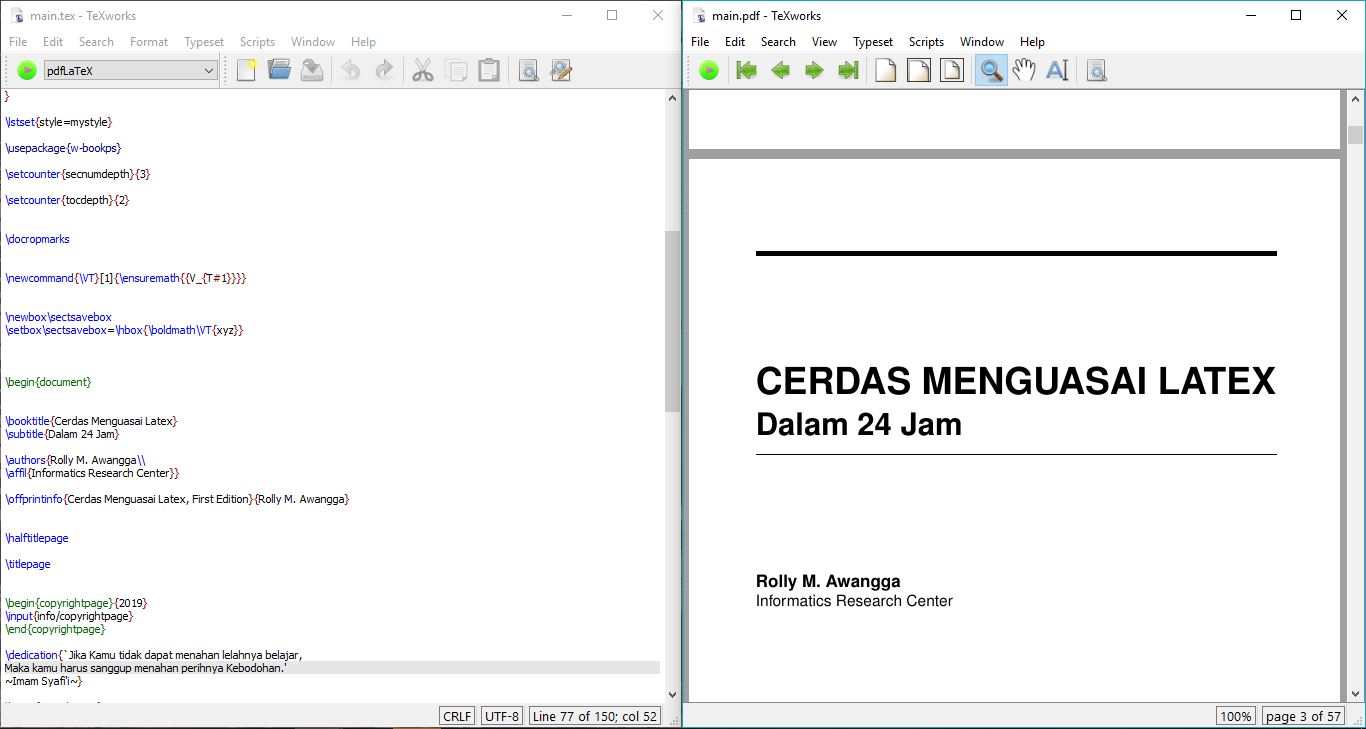
\includegraphics[width=.75\textwidth]{figures/main.JPG}
  \caption{main.tex dan main.pdf}\label{fig:main}
\end{figure}
\item Setelah itu pastikan terlebih dahulu file dari chapter mana yang ingin kita rubah atau tambahkan
\item Buka file yang ingin kita edit pada direktori chapter seperti pada gambar \ref{fig:chapter}
\begin{figure}[!htbp]
  \centering
  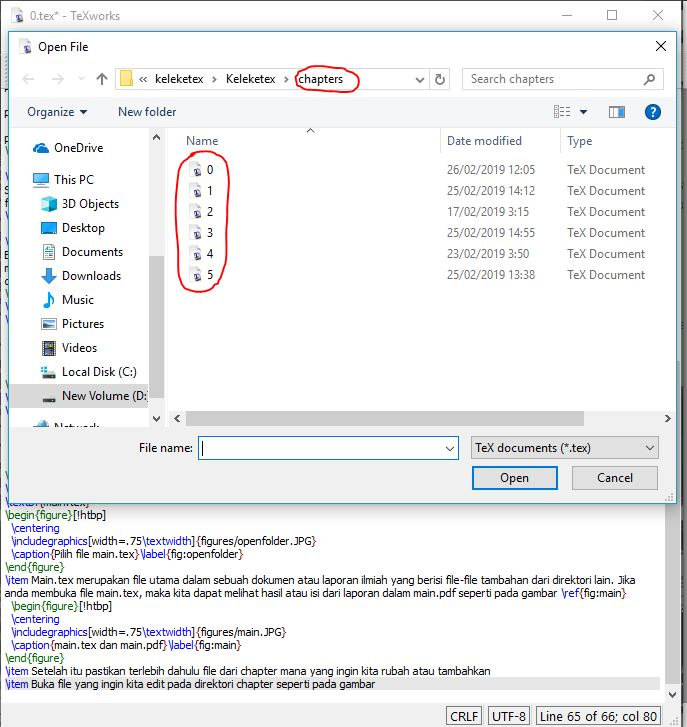
\includegraphics[width=.75\textwidth]{figures/chapter.JPG}
  \caption{Pilih chapter yang ingin di edit}\label{fig:chapter}
\end{figure}
\item Setelah membuka chapter yang ingin kita rubah, edit chapter tersebut sesuai kebutuhan
\item Pastikan kembali tidak ada perintah yang menyimpang ketika mengedit chapter tersebut 
\item Jika anda telah selesai melakukan pengeditan, pilih menu file lalu klik save all seperti pada gambar \ref{fig:saveall}
\begin{figure}[!htbp]
  \centering
  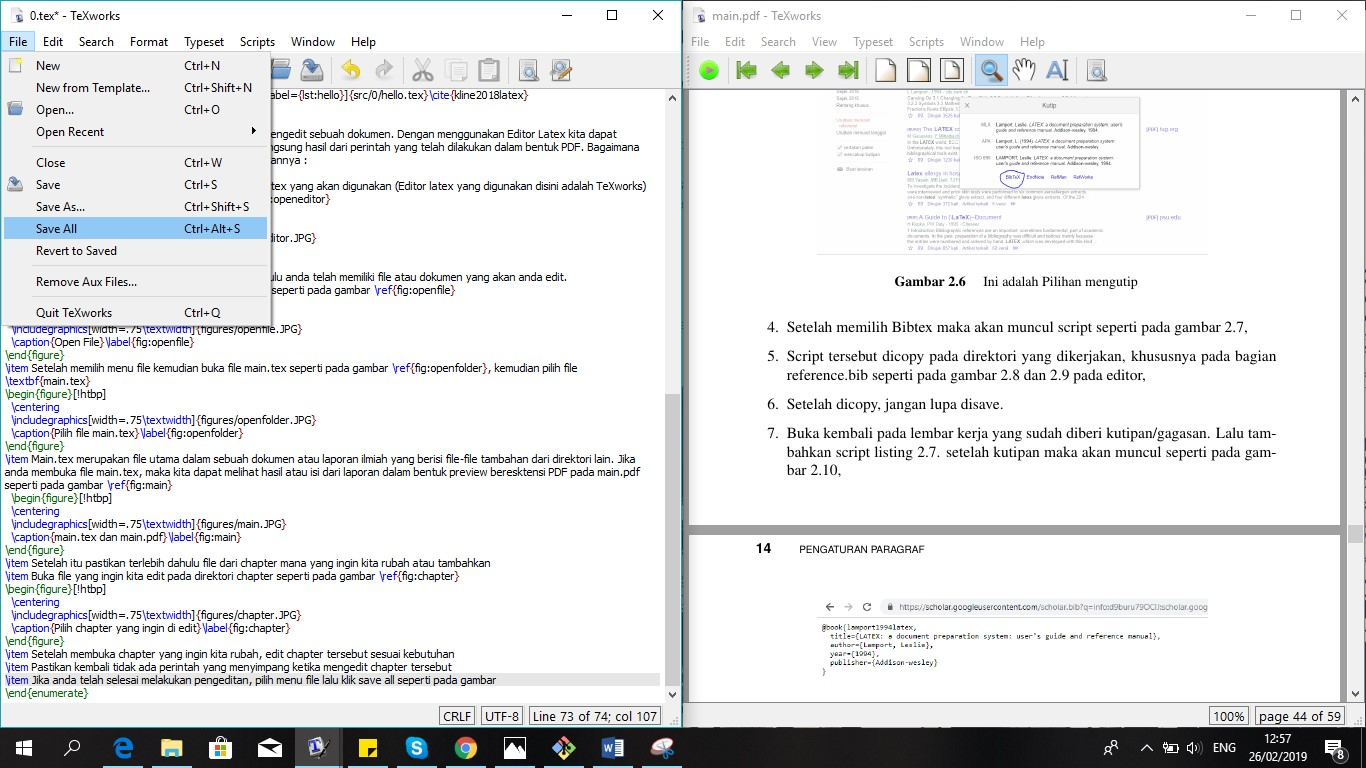
\includegraphics[width=.75\textwidth]{figures/saveall.JPG}
  \caption{Pilih Save all}\label{fig:saveall}
\end{figure}
\item Setelah itu agar perintah yang telah kita buat dapat dijalankan, buka kembali main.tex lalu pilih button \textit{typeset} dengan format \textit{pdflatex} untuk melakukan compile  seperti pada gambar \ref{fig:compile}
 \begin{figure}[!htbp]
  \centering
  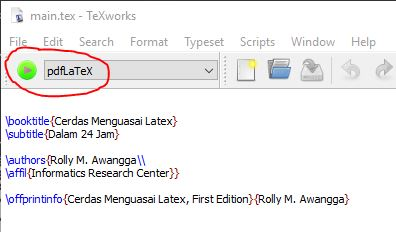
\includegraphics[width=.75\textwidth]{figures/compile.JPG}
  \caption{Proses Melakukan Compile}\label{fig:compile}
\end{figure}
\item Setelah melakukan compile pastikan kembali tidak ada perintah yang error pada \textit{console output}nya seperti pada gambar \ref{fig:cnpt}
\begin{figure}[!htbp]
  \centering
  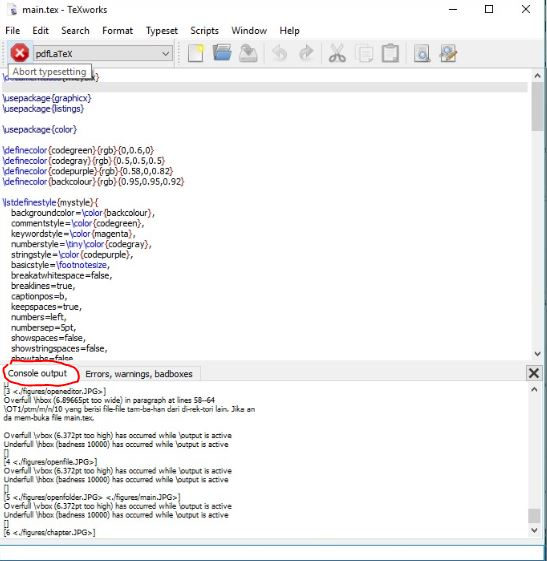
\includegraphics[width=.75\textwidth]{figures/cnpt.JPG}
  \caption{Console Output}\label{fig:cnpt}
\end{figure}
\item Jika terjadi error kita dapat melihat error tersebut dan memperbaikinya pada bagian \textit{Error,Warnings,Badboxes} seperti pada gambar \ref{fig:error}
\begin{figure}[!htbp]
  \centering
  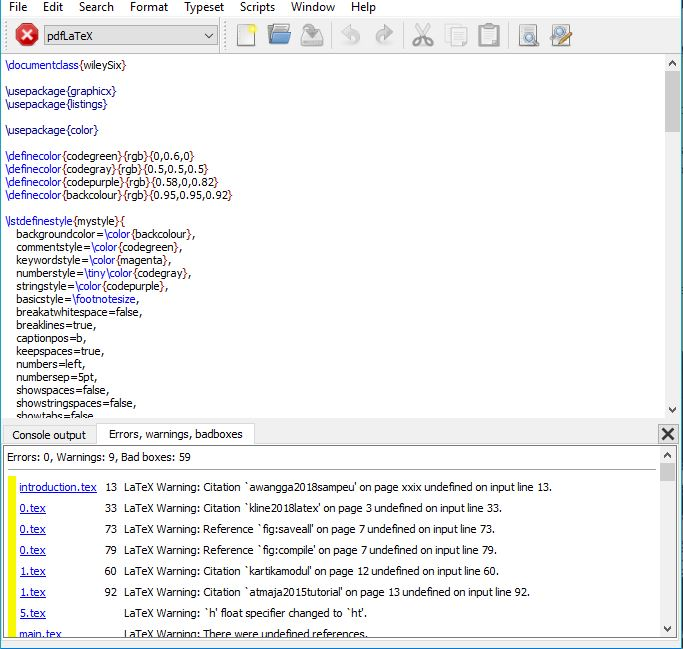
\includegraphics[width=.75\textwidth]{figures/error.JPG}
  \caption{Errors}\label{fig:error}
\end{figure}
\end{enumerate}